\documentclass[../main.tex]{subfiles}

\begin{document}
    \subsection{Definicje.}

    \textbf{Definicja testowania jest niejednoznaczna:}
    \begin{itemize}
        \item Testowanie to wykonywanie oprogramowania z intencją wykrywania
        tkwiących w nim błędów.
        \item Testowanie to krytyczne sprawdzanie, obserwacja i ewaluacja jakości
        oprogramowania.
        \item Testowanie to proces analizowania fragmentu oprogramowania w celu
        wykrycia różnic pomiędzy istniejącymi a pożądanymi warunkami (czyli
        defektów) oraz w celu oceny cech tego fragmentu oprogramowania [IEEE].
    \end{itemize}

    \begin{figure}[H]
        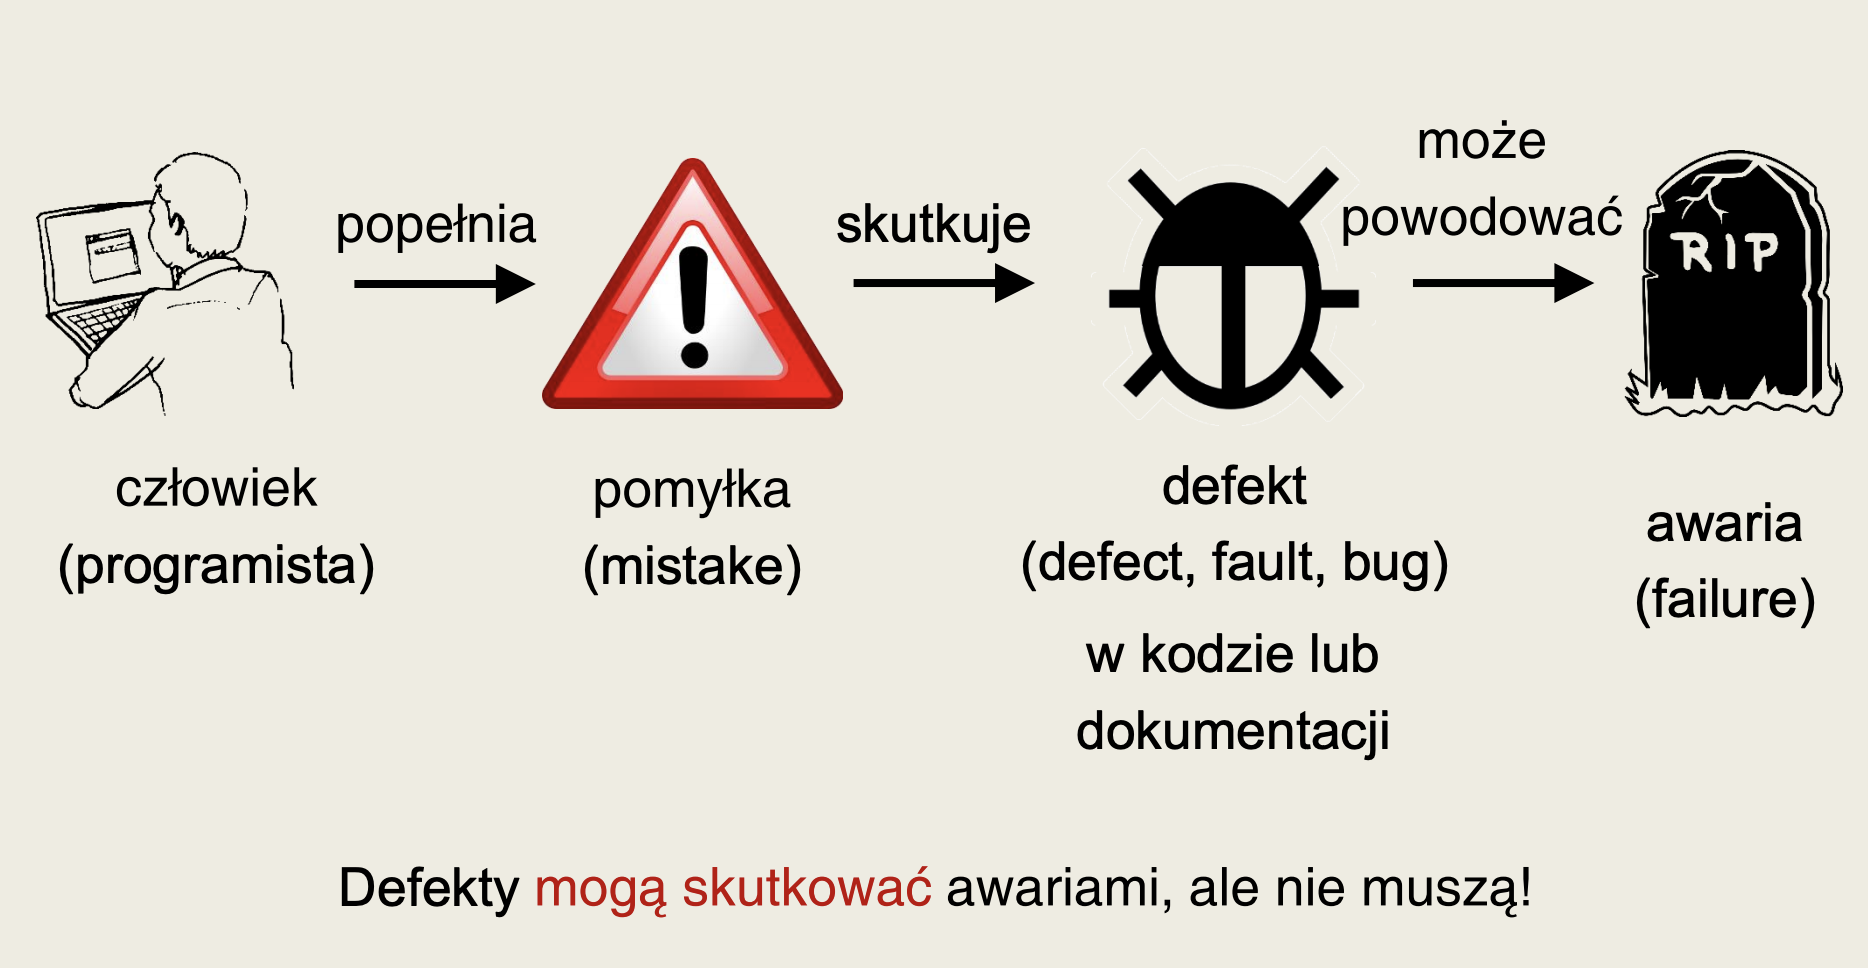
\includegraphics[width=\linewidth]{definicje.png}
    \end{figure}

    \textbf{Pomyłka} - człowiek robi coś źle.

    \textbf{Defekt (usterka, bug, fault)} - statyczny defekt w kodzie (lub dokumentacji), skutek pomyłki człowieka.

    \textbf{Błąd (error)} – nieprawidłowy stan wewnętrzny programu
    np. licznik pętli ustawiony na drugim zamiast pierwszym elemencie tablicy.

    \textbf{Awaria (failure)} – widoczne, nieprawidłowe działanie oprogramowania
    np. crash systemu, zwrócenie nieprawidłowego wyniku, komunikat o błędzie.

    \textbf{Walidacja (validation)} – ewaluacja oprogramowania w
    końcowej fazie procesu budowy, dokonywana w celu
    potwierdzenia zgodności z założonymi celami użycia (\textbf{are we building the right thing?}).


    \textbf{Weryfikacja (verification)} – ewaluacja we wczesnych fazach,
    sprawdzająca, czy produkt danej fazy spełnia wymagania
    (zwykle techniczne) ustalone podczas poprzedniej fazy (\textbf{are we building the thing right?}).

    \subsubsection{Debugowanie.}

    \textbf{Testowanie to nie debugowanie.}

    \textbf{Testowanie znajduje} awarie.

    \textbf{Debugowanie}, na podstawie informacji o awarii:
    \begin{itemize}
        \item \textbf{lokalizuje miejsce usterki} powodującej tę awarię
        \item usuwa (\textbf{naprawia}) usterkę
    \end{itemize}

    \textbf{Testowanie sprawdza}, czy usterka została poprawnie usunięta.

    \subsection{Rola testowania.}
    \begin{itemize}
        \item dobrze zaprojektowany, zdany test
        redukuje poziom ryzyka
        \item testowanie zwiększa przekonanie o
        jakości jeśli znajduje mało defektów
        lub nie znajduje ich w ogóle
        \item \textbf{jakość systemu} wzrasta gdy defekty są naprawiane
        \item wymagania kontraktowe i prawne, standardy przemysłowe
        \item jedna z czynności \textbf{QA} - Quality Assurance.
    \end{itemize}

    \subsection{Cele testowania.}
    \begin{itemize}
        \item znajdowanie defektów (np. testy jednostkowe)
        \item uzyskanie pewności co do poziomu jakości (np. testy akceptacyjne)
        \item dostarczenie informacji do podjęcia decyzii (np. ocena jakości systemu)
        \item zapobieganie pojawiania się defektów (np. projektowanie testów we wczesnych fazach życia)
    \end{itemize}

    Decyzja o zakresie i ilości testów zależy od \textbf{ryzyka} (ryzyko techniczne, biznesowe i safety risk)
    oraz \textbf{ograniczeń projektowych} (czas, budżet).


    \subsection{7 uniwersalnych zasad testowania.}
    \begin{enumerate}
        \item Testowanie ujawnia usterki
        \item Testowanie gruntowne jest niewykonalne
        \item Wczesne testowanie
        \item Kumulowanie się błędów
        \item Paradoks pestycydów
        \item Testowanie zależy od kontekstu
        \item Mylne przekonanie o braku błędów
    \end{enumerate}

    \subsection{Normy i standardy związanie z testowaniem}
    \begin{itemize}
        \item \textbf{IEEE 829} – dokumentacja testowa
        \item \textbf{IEEE 1008} – standard dla testowania jednostkowego
        \item \textbf{IEEE 1028} – standard dla przeglądów i audytów
        \item \textbf{ISO 9126} – model jakości (stara)
        \item \textbf{ISO/IEEE 25000} – model jakości (nowa)
        \item \textbf{ISO/IEEE 29119} – Software Testing Standard
    \end{itemize}


    Suita testowa - ????
\end{document}